\documentclass[11pt]{article}

\usepackage[margin=1in]{geometry}
\usepackage{setspace}
\setstretch{1.02}
\usepackage{booktabs}
\usepackage{graphicx}
\usepackage{caption}
\usepackage{longtable}
\usepackage{float}
\usepackage{amsmath}
\usepackage{amssymb}
\usepackage{xcolor}
\usepackage{array}
\usepackage[hidelinks]{hyperref}
\hypersetup{pdftitle={Training-Free Token Reduction on MotionBench: Benchmark Results},
            pdfauthor={HuVLLM Project}}

\captionsetup{font=small,labelfont=bf}

\title{Training-Free Token Reduction on MotionBench\\
\large Benchmark Results for Eleven Methods across Two Backbones}
\author{HuVLLM Project}
\date{\today}

\begin{document}
\maketitle

\begin{abstract}
This report presents benchmark results for eleven training-free video-LLM
token-reduction methods on MotionBench (8{,}052 questions, 4{,}018
scoreable), evaluated on two backbones at a standardized 32 frames and 15\%
nominal token retention. Headline numbers: the Qwen3-VL-8B baseline reaches
62.52\% against LLaVA-OV-7B's 52.66\%, a 9.86-point gap that holds across
all six question categories. On LLaVA-OV no method differs from its backbone
by more than the $\pm1.54$-point resolution floor except two that collapse
to 36.78\% and 38.20\%. On Qwen3-VL, at identical settings, all ten portable
methods lose accuracy, ranging from $-0.35$ to $-6.55$, and eight of those
losses are statistically significant. Results are reported overall and by
category; methodology, verification, and limitations are in the appendices.
\end{abstract}

\tableofcontents

% =====================================================================
\section{Setup}
\label{sec:setup}

\paragraph{Benchmark.} MotionBench: 8{,}052 four-option multiple-choice
questions over video clips. 4{,}034 carry an \texttt{NA} ground truth and
are excluded, leaving \textbf{4{,}018 scoreable items} --- the denominator
for every accuracy figure below. Six question categories, of unequal size
(Table~\ref{tab:baseline}). Scoring letter-matches A--D against ground
truth; generation is greedy.

\paragraph{Backbones.} \textbf{LLaVA-OV-7B} (SigLIP-so400m vision tower,
Qwen2-7B LLM, mid-2024) and \textbf{Qwen3-VL-8B}
(\texttt{Qwen3VLForConditionalGeneration}, a native architecture rather than
a LLaVA derivative, late-2025).\footnote{Project records refer to a
\texttt{qwen\_1\_5} template on LLaVA-OV. That is a prompt template, not a
different LLM: \texttt{qwen\_1\_5} and \texttt{qwen\_2} render
byte-identical prompts here and the model is Qwen2-7B either way.}

\paragraph{Configuration.} All methods run at 32 frames. Methods exposing a
single retention parameter are set to 15\%; those whose budget is fixed
internally, or that select frames rather than tokens, keep published
defaults. Comparison is therefore at a common \emph{nominal} setting, not at
equal compute --- measured budgets range from 7.5\% to 50\%
(Appendix~\ref{app:budget}).

\paragraph{Reading the numbers.} At $n=4{,}018$ the binomial 95\%
confidence half-width is $\pm1.54$ points; smaller differences are not
resolvable and are not ranked. $^{*}$ marks a difference significant by
McNemar's test on paired predictions ($\chi^2\geq3.84$, $p<0.05$); paired
counts are in Appendix~\ref{app:verification}. Every figure here was
recomputed from per-sample prediction records
(Appendix~\ref{app:provenance}).

% =====================================================================
\section{Results}
\label{sec:results}

\subsection{Summary}
\label{sec:summary}

\begin{table}[H]
  \centering
  \small
  \caption{All methods on both backbones, sorted by Qwen3-VL result.
  $^{*}$ = significant vs.\ that backbone's baseline. Dashes mark cells not
  independently recomputed for this report (see
  Appendix~\ref{app:provenance}) or not applicable.}
  \label{tab:summary}
  \begin{tabular}{lrrrr}
    \toprule
    & \multicolumn{2}{c}{LLaVA-OV-7B} & \multicolumn{2}{c}{Qwen3-VL-8B} \\
    \cmidrule(lr){2-3}\cmidrule(lr){4-5}
    Method & Overall & $\Delta$ & Overall & $\Delta$ \\
    \midrule
    \textit{Baseline} & \textit{52.66} & --- & \textit{62.52} & --- \\
    \midrule
    PruneVID$^{\dagger}$ & 38.20 & --14.46$^{*}$ & 62.17 & --0.35 \\
    DyCoke & 53.36 & +0.70 & 61.85 & --0.67 \\
    HoliTom & 53.14 & +0.47 & 60.33 & --2.19$^{*}$ \\
    MDP3 & --- & --- & 59.66 & --2.86$^{*}$ \\
    FastV$^{\dagger}$ & 36.78 & --15.88$^{*}$ & 59.01 & --3.51$^{*}$ \\
    VisionZip (ctx.)$^{\ddagger}$ & --- & --- & 58.81 & --3.71$^{*}$ \\
    STTM & --- & --- & 57.07 & --5.45$^{*}$ \\
    FlashVID & 53.31 & +0.65 & 56.65 & --5.87$^{*}$ \\
    VideoITG & --- & --- & 56.35 & --6.17$^{*}$ \\
    AIM & --- & --- & 55.97 & --6.55$^{*}$ \\
    \bottomrule
  \end{tabular}
\end{table}

\noindent\footnotesize
$^{\dagger}$ These two LLaVA-OV results are under review: both collapse with
matched signatures and share one code path, and a control experiment
separating method from harness has not yet reported (\S\ref{sec:collapse},
Appendix~\ref{app:open}). \quad
$^{\ddagger}$ Contextual half only --- Qwen3-VL's vision tower has no CLS
token, so VisionZip's dominant half is not implementable. Not the published
method. VisionZip's complete form runs on LLaVA-1.5-7B
(Table~\ref{tab:native}). \quad
DyTo appears in Table~\ref{tab:native}: it is bound to a Vicuna backbone and
runs on neither of these two.\normalsize

\medskip

Table~\ref{tab:summary} contains the report's main observation. Reading
across rows rather than down columns, the ordering does not survive the
change of backbone: PruneVID is the worst result on LLaVA-OV and the best on
Qwen3-VL; FlashVID is indistinguishable from the backbone on LLaVA-OV and
loses 5.87 points on Qwen3-VL. Every Qwen3-VL delta is negative; three of
five LLaVA-OV deltas are positive but none resolvably so.

\subsection{Backbones}
\label{sec:backbone}

\begin{table}[H]
  \centering
  \small
  \caption{Baseline accuracy overall and by category (\% correct within
  category). AO = Action Order, CM = Camera Motion, LM = Location-related
  Motion, MR = Motion Recognition, MO = Motion-related Objects,
  RC = Repetition Count. Chance is 25\%.}
  \label{tab:baseline}
  \begin{tabular}{lrrrrrrr}
    \toprule
    Backbone & Overall & AO & CM & LM & MR & MO & RC \\
    \midrule
    LLaVA-OV-7B & 52.66 & 40.5 & 45.2 & 55.5 & 57.0 & 71.2 & 23.8 \\
    Qwen3-VL-8B & 62.52 & 46.1 & 63.1 & 65.0 & 67.3 & 79.0 & 33.8 \\
    \midrule
    $\Delta$ & +9.86 & +5.6 & +17.9 & +9.5 & +10.3 & +7.8 & +10.0 \\
    \midrule
    $n$ & 4{,}018 & 519 & 385 & 546 & 1{,}478 & 690 & 400 \\
    \bottomrule
  \end{tabular}
\end{table}

\begin{figure}[htbp]
  \centering
  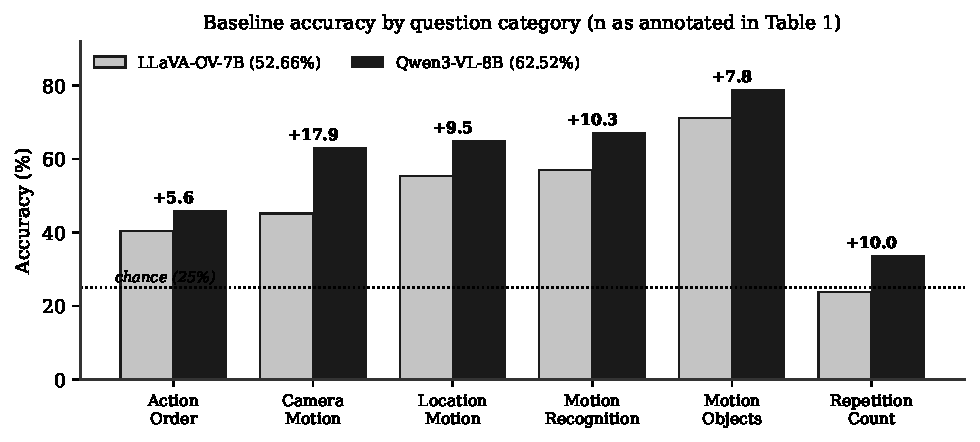
\includegraphics[width=0.86\linewidth]{figures/fig1_baseline_profile.pdf}
  \caption{Baseline accuracy by category. Qwen3-VL-8B leads in all six,
  most sharply on Camera Motion ($+17.9$).}
  \label{fig:baseline}
\end{figure}

The 9.86-point backbone gap is larger than any method effect measured
anywhere in this report, and it holds in every category.

Two properties of Table~\ref{tab:baseline} govern how later tables should be
read. Both backbones are strongest on Motion-related Objects (71.2\%,
79.0\%), the category most answerable from object appearance without
integrating motion. And \textbf{Repetition Count is at or near chance for
both} (23.8\% and 33.8\% against 25\%): LLaVA-OV is not distinguishable from
guessing there, so movement in that column is not evidence about a method
and is not interpreted below.

\subsection{LLaVA-OV-7B}
\label{sec:llava}

\begin{table}[H]
  \centering
  \small
  \caption{LLaVA-OV-7B, 32 frames, 15\% nominal retention. Categories as in
  Table~\ref{tab:baseline}. VisionZip runs on a different backbone
  (Table~\ref{tab:native}); MDP3, AIM, VideoITG and STTM are not included
  here (Appendix~\ref{app:provenance}).}
  \label{tab:llava}
  \begin{tabular}{lrrrrrrrr}
    \toprule
    Method & Overall & $\Delta$ & AO & CM & LM & MR & MO & RC \\
    \midrule
    DyCoke & 53.36 & +0.70 & 38.9 & 48.8 & 55.7 & 58.2 & 70.9 & 25.2 \\
    FlashVID & 53.31 & +0.65 & 39.9 & 45.7 & 53.8 & 58.0 & 71.7 & 28.2 \\
    HoliTom & 53.14 & +0.47 & 40.8 & 49.6 & 52.6 & 57.0 & 71.4 & 27.3 \\
    \textit{Baseline} & \textit{52.66} & --- & \textit{40.5} & \textit{45.2} & \textit{55.5} & \textit{57.0} & \textit{71.2} & \textit{23.8} \\
    PruneVID-OV$^{*\dagger}$ & 38.20 & --14.46 & 32.0 & 34.8 & 35.5 & 38.4 & 52.9 & 27.3 \\
    FastV$^{*\dagger}$ & 36.78 & --15.88 & 32.8 & 31.9 & 34.1 & 35.7 & 53.8 & 25.2 \\
    \bottomrule
  \end{tabular}
\end{table}

DyCoke, FlashVID and HoliTom land within 0.70 points of the backbone, inside
the $\pm1.54$-point floor, none significant (largest $\chi^2 = 2.34$ against
a 3.84 threshold). They are statistically indistinguishable from the
backbone and from each other; the ordering among them is not meaningful.
Their category profiles track the backbone closely, with the largest
deviations falling in the two smallest categories.

FastV and PruneVID-OV lose more than 14 points each, significantly, and
degrade in every category carrying above-chance backbone signal
(\S\ref{sec:collapse}).

\subsection{Qwen3-VL-8B}
\label{sec:qwen}

\begin{table}[H]
  \centering
  \small
  \caption{Qwen3-VL-8B, 32 frames, 15\% nominal retention. All ten portable
  methods. VisionZip is the contextual half only (see
  Table~\ref{tab:summary} notes).}
  \label{tab:qwen}
  \begin{tabular}{lrrrrrrrr}
    \toprule
    Method & Overall & $\Delta$ & AO & CM & LM & MR & MO & RC \\
    \midrule
    \textit{Baseline} & \textit{62.52} & --- & \textit{46.1} & \textit{63.1} & \textit{65.0} & \textit{67.3} & \textit{79.0} & \textit{33.8} \\
    PruneVID & 62.17 & --0.35 & 46.1 & 62.9 & 64.1 & 67.1 & 79.1 & 32.5 \\
    DyCoke & 61.85 & --0.67 & 45.1 & 62.6 & 63.9 & 66.4 & 78.4 & 34.5 \\
    HoliTom$^{*}$ & 60.33 & --2.19 & 44.7 & 61.3 & 61.0 & 66.4 & 76.2 & 29.0 \\
    MDP3$^{*}$ & 59.66 & --2.86 & 44.9 & 64.7 & 62.8 & 64.0 & 77.4 & 23.0 \\
    FastV$^{*}$ & 59.01 & --3.51 & 46.2 & 61.0 & 61.9 & 63.5 & 72.2 & 30.5 \\
    VisionZip (ctx.)$^{*}$ & 58.81 & --3.71 & 43.2 & 57.4 & 61.9 & 64.2 & 74.3 & 29.5 \\
    STTM$^{*}$ & 57.07 & --5.45 & 44.3 & 60.0 & 61.0 & 60.6 & 73.8 & 23.8 \\
    FlashVID$^{*}$ & 56.65 & --5.87 & 43.4 & 57.9 & 57.1 & 61.2 & 73.0 & 27.0 \\
    VideoITG$^{*}$ & 56.35 & --6.17 & 45.3 & 53.5 & 59.3 & 60.2 & 75.4 & 22.2 \\
    AIM$^{*}$ & 55.97 & --6.55 & 45.9 & 56.6 & 59.5 & 58.3 & 72.2 & 27.0 \\
    \bottomrule
  \end{tabular}
\end{table}

\begin{figure}[htbp]
  \centering
  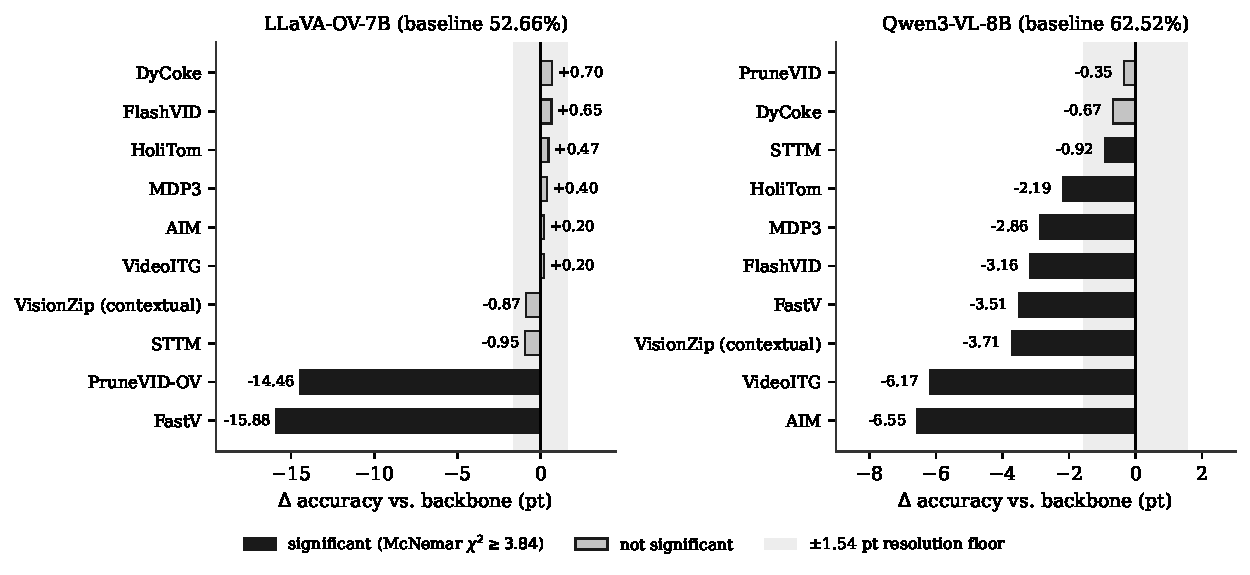
\includegraphics[width=\linewidth]{figures/fig2_delta_both.pdf}
  \caption{Change vs.\ backbone on each model. Shaded band is the
  $\pm1.54$-point resolution floor. On LLaVA-OV every non-collapsed method
  falls inside it; on Qwen3-VL eight of ten fall outside it and all ten are
  negative.}
  \label{fig:delta}
\end{figure}

Every method loses accuracy on Qwen3-VL and eight of ten lose significantly.
The two exceptions, PruneVID ($-0.35$) and DyCoke ($-0.67$), are the two
that retain roughly half their tokens against 7.5--15\% for the rest
(Appendix~\ref{app:budget}).

Loss does not track budget monotonically. HoliTom operates at the smallest
measured budget in the set (7.5\%) and loses 2.19 points, while AIM and
FlashVID at 15\% lose 6.55 and 5.87. The methods that hold up are those that
merge non-retained tokens into survivors rather than discarding them
outright.

\subsection{Per-category change}
\label{sec:category}

\begin{figure}[htbp]
  \centering
  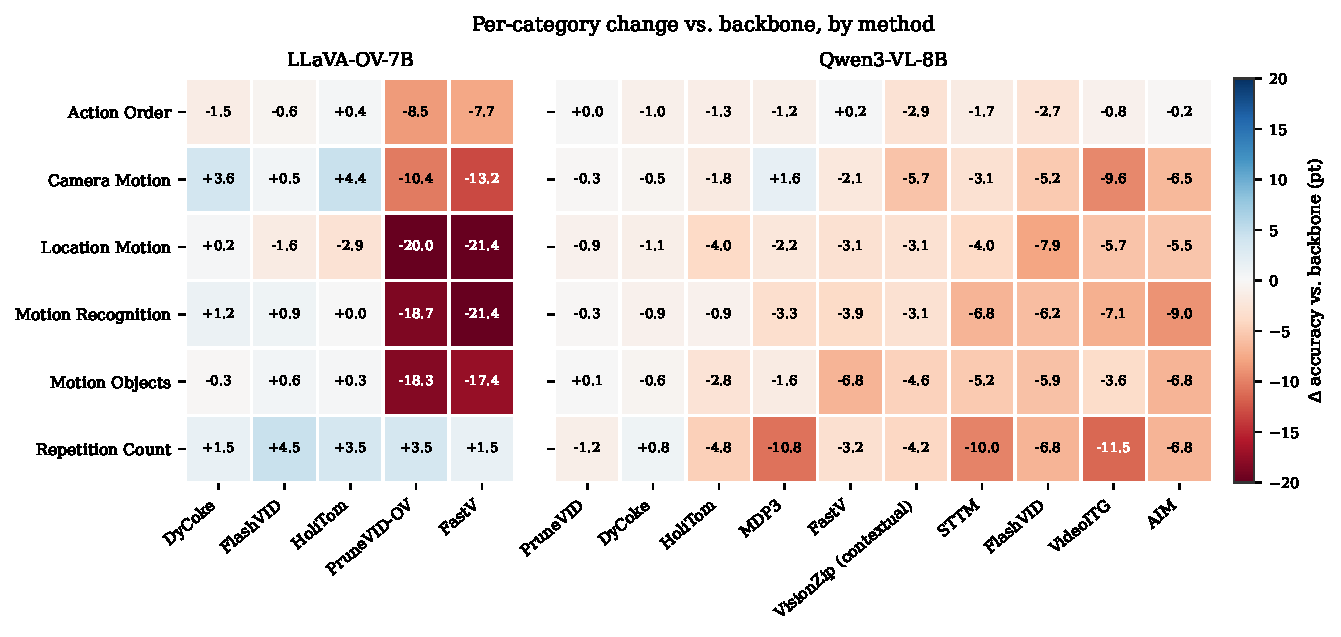
\includegraphics[width=\linewidth]{figures/fig3_category_delta.pdf}
  \caption{Per-category change vs.\ backbone, columns ordered by overall
  delta. Repetition Count movement is not interpretable --- both backbones
  are at or near chance there (Table~\ref{tab:baseline}).}
  \label{fig:catdelta}
\end{figure}

Losses are not spread evenly across question types. Expressing retained
above-chance signal as $(\text{method}-25)/(\text{backbone}-25)$, FastV on
LLaVA-OV keeps \textbf{62\%} of the backbone's above-chance signal on
Motion-related Objects but only \textbf{30\%} on Location-related Motion,
33\% on Motion Recognition and 34\% on Camera Motion. PruneVID-OV shows the
same ordering (60\% on Motion-related Objects, 34\% on Location-related
Motion). Motion-related Objects is the category most answerable from
appearance in isolated frames; categories requiring integration across
frames retain roughly half as much.

The pattern is milder but present on Qwen3-VL (Figure~\ref{fig:catdelta},
right), where the largest losses fall on Motion Recognition ($-9.0$, AIM)
and Camera Motion ($-9.6$, VideoITG), while Action Order moves within
$\pm3$ points for every method.

Repetition Count is the control column. LLaVA-OV scores 23.8\% there against
25\% chance, so there is no signal to preserve; the apparent gains under
FastV ($+1.5$) and PruneVID-OV ($+3.5$) accompany 15-point overall collapses
and reflect answer redistribution (\S\ref{sec:collapse}), not recovered
capability.

\subsection{Retention sweep}
\label{sec:retention}

\begin{table}[H]
  \centering
  \small
  \caption{Accuracy (and $\Delta$ vs.\ backbone) across nominal retention,
  32 frames and all else fixed. Span is movement from 10\% to 25\%. Four of
  eleven methods expose a comparable retention parameter.}
  \label{tab:retention}
  \begin{tabular}{lrrrr}
    \toprule
    Method & $r=0.10$ & $r=0.15$ & $r=0.25$ & Span \\
    \midrule
    \multicolumn{5}{l}{\textit{LLaVA-OV-7B (baseline 52.66\%)}} \\
    FastV & 36.06 (--16.60)$^{*}$ & 36.78 (--15.88)$^{*}$ & 36.73 (--15.93)$^{*}$ & +0.67 \\
    FlashVID & 52.51 (--0.15) & 53.31 (+0.65) & 53.36 (+0.70) & +0.85 \\
    HoliTom & 52.76 (+0.10) & 53.14 (+0.47) & 53.41 (+0.75) & +0.65 \\
    PruneVID & 38.10 (--14.56)$^{*}$ & 38.20 (--14.46)$^{*}$ & 38.38 (--14.29)$^{*}$ & +0.28 \\
    \midrule
    \multicolumn{5}{l}{\textit{Qwen3-VL-8B (baseline 62.52\%)}} \\
    FastV & 56.92 (--5.60)$^{*}$ & 59.01 (--3.51)$^{*}$ & 60.60 (--1.92)$^{*}$ & \textbf{+3.68} \\
    FlashVID & 54.73 (--7.79)$^{*}$ & 56.65 (--5.87)$^{*}$ & 59.36 (--3.16)$^{*}$ & \textbf{+4.63} \\
    HoliTom & 60.05 (--2.46)$^{*}$ & 60.33 (--2.19)$^{*}$ & 60.43 (--2.09)$^{*}$ & +0.38 \\
    PruneVID & 60.23 (--2.29)$^{*}$ & 62.17 (--0.35) & 61.40 (--1.12)$^{*}$ & +1.17 \\
    \bottomrule
  \end{tabular}
\end{table}

\begin{figure}[htbp]
  \centering
  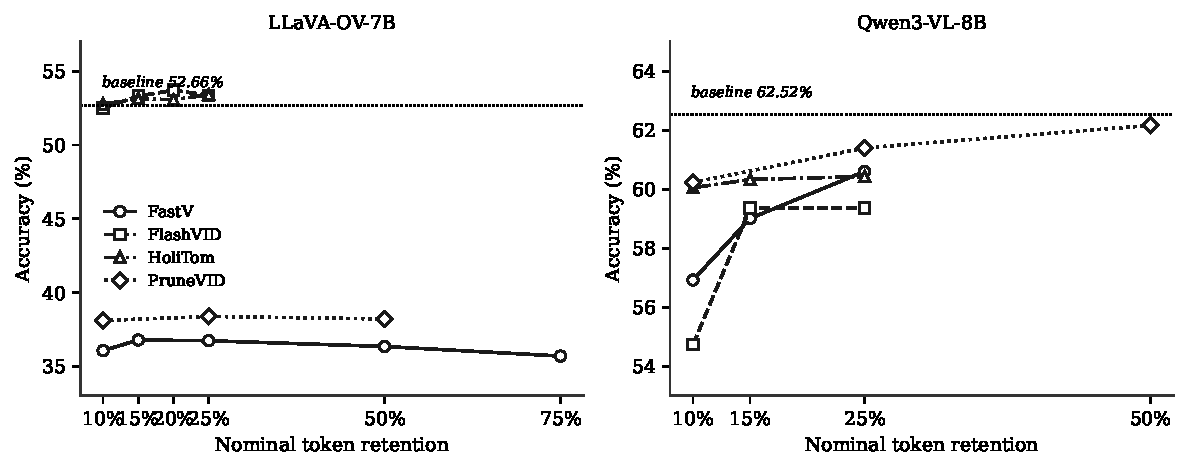
\includegraphics[width=\linewidth]{figures/fig4_retention.pdf}
  \caption{Accuracy against nominal token retention. On LLaVA-OV the four
  methods occupy two flat regimes the budget does not move; on Qwen3-VL the
  same methods respond strongly to the same parameter.}
  \label{fig:retention}
\end{figure}

Tripling the budget from 10\% to 25\% moves no LLaVA-OV method more than
0.85 points. On Qwen3-VL the same change moves FlashVID 4.63 points and
FastV 3.68, with FastV's significance decaying monotonically
($\chi^2 = 89.8 \to 44.6 \to 18.2$) as it converges toward the baseline ---
roughly a five-fold difference in retention sensitivity between the two
backbones.

On LLaVA-OV the four methods sit in two flat regimes: FlashVID and HoliTom
at the baseline at every setting, FastV and PruneVID roughly 15 points below
it at every setting. What costs accuracy there is that those two prune at
all, not how hard.

One cell is flagged rather than smoothed: PruneVID on Qwen3-VL is
non-monotonic ($60.23 \to 62.17 \to 61.40$), its midpoint both its best
result and its only non-significant one. At $\pm1.54$-point resolution this
may be noise; it is not reported as a trend.

\subsection{Answer distribution on LLaVA-OV}
\label{sec:collapse}

\begin{table}[H]
  \centering
  \small
  \caption{Distribution of predicted answer letters on LLaVA-OV-7B, \% of
  4{,}018 scoreable items.}
  \label{tab:answers}
  \begin{tabular}{lrrrr}
    \toprule
    Run & A & B & C & D \\
    \midrule
    \textit{Ground truth} & \textit{25.4} & \textit{25.6} & \textit{25.5} & \textit{23.6} \\
    Baseline & 27.1 & 26.6 & 26.9 & 19.3 \\
    DyCoke & 27.4 & 26.1 & 27.0 & 19.3 \\
    FlashVID & 27.7 & 25.6 & 25.7 & 20.8 \\
    HoliTom & 26.1 & 24.1 & 27.2 & 22.5 \\
    PruneVID-OV & 12.2 & 26.7 & 15.0 & \textbf{46.0} \\
    FastV & 14.9 & 23.0 & 15.2 & \textbf{46.7} \\
    \bottomrule
  \end{tabular}
\end{table}

The two collapsed methods place 46--47\% of their answers on option D
against a 23.6\% ground-truth rate, while the backbone and the three
merge-based methods stay near uniform. This is the behaviour of a model
answering from the prompt without usable visual evidence, and it explains
the apparent Repetition Count gains in \S\ref{sec:category}: a near-uniform
category rewards a degenerate constant answer at roughly chance.

The signature is retention-invariant. Across $r \in \{0.10, 0.15, 0.25\}$
FastV's D-rate is 47.0\%, 46.8\%, 47.1\% --- flat to a tenth of a point
while accuracy moves 0.67 points. Restoring tokens does not restore visual
grounding on this backbone, though it does for the same algorithm on
Qwen3-VL, where the answer distribution tracks the backbone within 1.5
points at every budget.

\paragraph{Caveat on these two rows.} FastV and PruneVID-OV are different
algorithms at different layers with different selection rules, yet fail with
signatures matching to about one point on accuracy, D-rate, broken/fixed
ratio and flatness across retention. Both LLaVA-OV ports drive reduction
through the same code path. A control experiment separating algorithm from
harness is queued and has not reported; until it does, these two rows are
reported as measurements of this harness and their attribution to the
published methods is open (Appendix~\ref{app:open}).

\subsection{Methods on non-standard backbones}
\label{sec:native}

\begin{table}[H]
  \centering
  \small
  \caption{Runs on backbones other than the two standardized ones. Not
  comparable to Tables~\ref{tab:llava}--\ref{tab:qwen}; no $\Delta$ is given
  because no matched baseline exists for either row.}
  \label{tab:native}
  \begin{tabular}{llrrrrrrr}
    \toprule
    Method & Backbone & Overall & AO & CM & LM & MR & MO & RC \\
    \midrule
    VisionZip & LLaVA-1.5-7B & 40.09 & 33.7 & 33.0 & 37.2 & 41.1 & 57.4 & 25.8 \\
    DyTo (recon.\ TW-FINCH) & Vicuna-7B & 42.06 & 32.4 & 33.0 & 42.1 & 43.0 & 61.7 & 26.0 \\
    \bottomrule
  \end{tabular}
\end{table}

VisionZip patches \texttt{CLIPVisionTower}, which LLaVA-OV does not have, so
its complete form runs only on LLaVA-1.5-7B --- and at 8 frames rather than
32. The 40.09\% differs from Table~\ref{tab:llava} in both backbone and
frame count and is never placed in a LLaVA-OV comparison.

DyTo carries two caveats. It is not reproducible from its published
artifacts (the released code calls an argument absent from its own pinned
dependency, and a clustering helper has no return statement); the missing
return was recovered by transcription from a character-identical sibling
function, but the temporal weighting had to be reimplemented, so the result
is reported only as ``DyTo (reconstructed TW-FINCH)''. And it is the one
number in this report with execution evidence but \textbf{no divergence
check}, because no baseline was ever run on its Vicuna backbone --- it is an
absolute score, not a measured method effect.

A token-matched control is documented in the project records (cited, not
recomputed here): against an uncompressed 6-frame baseline at 3{,}456 visual
tokens scoring 43.35\%, DyTo at $\sim$3{,}680 tokens scores 42.06\%, a
significant $-1.29$. A frame-matched control is impossible --- Vicuna's
4{,}096-token context cannot hold 32 uncompressed frames --- which is the
constraint DyTo exists to address.

% =====================================================================
\appendix
\newpage

\section{Methodology and verification}
\label{app:method}

\subsection*{The verification gate}
\label{app:gate}

A run that completes, reports a plausible accuracy, and did nothing is
indistinguishable from a successful one by accuracy alone. Every number in
this report therefore required two independent signals.

\textbf{1. Execution evidence.} The method's instrumentation reported a
token count consistent with its configured budget (Appendix~\ref{app:budget}).

\textbf{2. Prediction divergence from the unmodified backbone.} Greedy
decoding makes the pipeline a deterministic function of (weights, frames,
prompt): frame indices come from a fixed linear spacing, the vision tower is
frozen, token choice is $\arg\max$. Re-running an unchanged configuration
reproduces all 8{,}052 predictions exactly --- confirmed on three
independent run pairs, each diverging on 0 of 8{,}052. Against that zero
baseline, a method that discards or merges most of the visual input and
produces zero differing predictions cannot have executed.

The second signal is not redundant. Four ports passed every other check and
failed it: an early FastV integration whose pruning call was a stub; a
PruneVID port to LLaVA-OV whose discard mask was dropped before reaching the
model; and FlashVID and AIM on Qwen3-VL, which logged a correct budget
(\texttt{keep=1750 (15.0\%)}) while emitting byte-identical output, because
\texttt{attention\_mask} is \texttt{None} under this model's default
attention implementation and the mask-dependent path never ran. A fifth,
STTM on Qwen3-VL, failed because that model interleaves timestamp text
tokens between frames --- the 11{,}664 visual tokens occupy an 11{,}784-wide
span broken by 15 gaps, and a patch assuming one contiguous block did
nothing. All five would have entered the results tables as working methods
under an execution-log check alone.

\subsection*{Measured token budgets}
\label{app:budget}

\begin{table}[H]
  \centering
  \small
  \caption{Measured visual-token budget on Qwen3-VL-8B, read from each
  method's execution log rather than its CLI flag. Input is 11{,}664 visual
  tokens at 32 frames. Nominal 15\% describes five of ten methods.}
  \label{tab:budget}
  \begin{tabular}{llr}
    \toprule
    Method & Reduction stage & Measured budget \\
    \midrule
    HoliTom & pre-LLM segment retain $+$ in-LLM merge & 7.5\% (875 tokens) \\
    STTM & quadtree spatio-temporal merge & 9.0\% (1{,}050) \\
    FastV & in-LLM attention rerank, layer 2 & 15.0\% (1{,}750) \\
    FlashVID & pre-LLM temporal-segment merge & 15.0\% (1{,}750) \\
    AIM & bipartite merge $+$ PageRank prune & 15.0\% (1{,}750) \\
    VisionZip (contextual) & key-similarity merge in vision tower & 15.0\% (1{,}750) \\
    DyCoke & temporal merge $+$ KV prune, layer 3 & 49.0\% (5{,}716) \\
    PruneVID & DPC-KNN cluster merge, layer 10 & 50.0\% (5{,}832) \\
    \midrule
    MDP3 & frame selection (DPP) & 8 of 32 frames \\
    VideoITG & grounded frame selection & 32 of 512 sampled \\
    \bottomrule
  \end{tabular}
\end{table}

\subsection*{Provenance}
\label{app:provenance}

Every figure in the results tables and all four figures were recomputed for
this report directly from each run's per-sample prediction records, not
transcribed from prior documentation. Recomputed accuracy agreed with each
run's stored summary to within 0.01 points across all 42 available run
directories, and independently reproduced the documented divergence counts,
paired win/loss counts and per-category figures.

Four LLaVA-OV results --- MDP3 (53.06\%), AIM (52.86\%), VideoITG (52.86\%)
and STTM (51.72\%) --- are omitted from Table~\ref{tab:llava} and all
figures because their run directories were absent from the available cache;
only non-comparable sampled-decoding variants were present. They appear as
dashes in Table~\ref{tab:summary}. The DyTo token-matched control
(\S\ref{sec:native}) is cited on the same basis.

\section{Paired-prediction statistics}
\label{app:verification}

\emph{Differ} counts predictions unequal to the backbone's over all 8{,}052
rows (accuracy uses the 4{,}018 scoreable subset); 0 would indicate a silent
no-op. \emph{Fixed} and \emph{broke} are the McNemar discordant pairs on
scoreable items.

\begin{table}[H]
  \centering
  \small
  \caption{Paired-prediction statistics against each backbone.}
  \label{tab:verif}
  \begin{tabular}{lrrrrl}
    \toprule
    Method & Differ & Fixed & Broke & $\chi^2$ & Significant \\
    \midrule
    \multicolumn{6}{l}{\textit{LLaVA-OV-7B}} \\
    DyCoke & 1{,}031 & 170 & 142 & 2.34 & no \\
    FlashVID & 1{,}610 & 268 & 242 & 1.23 & no \\
    HoliTom & 1{,}838 & 299 & 280 & 0.56 & no \\
    PruneVID-OV & 4{,}536 & 473 & 1{,}054 & 220.30 & yes \\
    FastV & 4{,}605 & 475 & 1{,}113 & 255.52 & yes \\
    \midrule
    \multicolumn{6}{l}{\textit{Qwen3-VL-8B}} \\
    PruneVID & 1{,}074 & 56 & 70 & 1.34 & no \\
    DyCoke & 1{,}048 & 83 & 110 & 3.50 & no \\
    HoliTom & 1{,}657 & 131 & 219 & 21.63 & yes \\
    MDP3 & 1{,}626 & 159 & 274 & 30.01 & yes \\
    FastV & 2{,}029 & 149 & 290 & 44.65 & yes \\
    VisionZip (contextual) & 2{,}035 & 191 & 340 & 41.25 & yes \\
    STTM & 2{,}095 & 170 & 389 & 85.02 & yes \\
    FlashVID & 2{,}625 & 178 & 414 & 93.29 & yes \\
    VideoITG & 2{,}522 & 206 & 454 & 92.44 & yes \\
    AIM & 2{,}861 & 194 & 457 & 105.44 & yes \\
    \midrule
    \multicolumn{6}{l}{\textit{Backbone vs.\ backbone}} \\
    Qwen3-VL-8B vs.\ LLaVA-OV-7B & 7{,}081 & 942 & 546 & 127.47 & yes \\
    \bottomrule
  \end{tabular}
\end{table}

\section{Limitations}
\label{app:limits}

\textbf{Scope.} All results are on MotionBench and two backbones. Nothing
here generalizes to other video benchmarks; the per-category analysis of
\S\ref{sec:category} in fact predicts that these methods will look better on
benchmarks weighted toward appearance and object recognition.

\textbf{Single measurement per cell.} Greedy decoding makes each
configuration exactly reproducible, so there is one measurement per cell and
no run-to-run variance estimate. Reported uncertainty is binomial, not
empirical --- which is why the $\pm1.54$-point floor is applied strictly.

\textbf{Standardization is not paper fidelity.} FastV's published default is
$r=0.5$; the figures here are FastV \emph{at} 10--25\%, well outside its
validated range, and should not be read as characterizing the method as
published. Since methods without a retention knob keep their defaults, the
cross-method comparison is at a common nominal setting and not at equal
compute (Appendix~\ref{app:budget}).

\textbf{Determinism is conditional.} Bit-identical reproduction was verified
across nodes of the same GPU generation, same software stack, batch size 1.
Different GPU generations may perturb near-tied logits; that comparison was
not run. Replicators on other hardware should expect close, not identical,
numbers.

\textbf{Zero divergence is strong but not airtight.} A method pruning only
tokens the model already ignored would execute correctly and produce zero
divergence, and the gate would misclassify it. No such case was observed.

\textbf{Scoring protocol.} Accuracy depends on a letter-matching regular
expression and on excluding the 4{,}034 \texttt{NA} items --- roughly half
the benchmark. Both are documented choices; neither has been ablated.

\section{Open items}
\label{app:open}

\begin{enumerate}
\item \textbf{FastV and PruneVID-OV on LLaVA-OV: method or harness?} Both
  drive reduction through the same code path and fail with matched
  signatures. The decisive experiment is a \texttt{keepall} control that
  traverses that path while discarding nothing; if it does not return
  $\approx$52.66\%, both rows are harness artifacts and must be withdrawn
  and re-run. Four arms are queued and have not reported. The
  retention-invariance and answer-distribution evidence of
  \S\ref{sec:collapse} stands either way --- what is open is whether it
  describes the published methods or this integration of them.
\item \textbf{Sampled-decoding answer distribution.} A companion study under
  $\text{temperature}=0.7$, $\text{top-}p=0.9$ (not comparable to any gated
  result, since sampling defeats the divergence check) is missing its
  FlashVID row; that run is in flight.
\end{enumerate}

\end{document}
